\section{Application to Symmetry Groups of Regular Solids}
Let $S$ be a regular solid and $V$ its vertices.
The the symmetries of $S$ are the isometries (distance preserving maps) of $\mathbb{R}^2$ or $\mathbb{R}^3$ that maps $S$ to itself.
The dual is the solid with vertices in the middle of each face of the input.

\subsection{Tetrahedron (self-dual)}

\begin{figure}
    \centering 
    \includegraphics[height=5cm]{figures/07-tetrahedron}
\end{figure} faces are $4$ equilateral triangles.

Let $G$ be group of symmetries of $T$, and $X = \{\text{vertices of } T\} = \{1, 2, 3, 4\}$.
Then $\exists$ a homomorphism
\begin{align*}
    \Phi : G &\to \operatorname{Sym} X \cong S_4 \text{ \Cref{prp:6}}
\end{align*} 
Note $\ker \Phi = \{ e \}$, if all vertices are fixed, then $T$ fixed. \\
Consider $G^+ \leq G$ be the subgroup of all rotations.
The elements of $G^+$ are as follows:

\begin{figure}
    \centering 
    \includegraphics[height=5cm]{figures/07-tetrahedron-rotations} 
    \caption{Rotation of $2 \pi / 3$, a 3-cycle $\begin{pmatrix}2 & 3 & 4\end{pmatrix}$, and $4 \pi / 3$ gives $\begin{pmatrix}2 & 4 & 3\end{pmatrix}$.}
\end{figure}

There are $4$ such axes, giving $8$ rotations of order $3$ (these are all the $3$-cycles in $S_4$).

\begin{figure} 
    \centering 
    \includegraphics[height=5cm]{figures/07-tetrahedron-double-transposition} 
    \caption{Rotation of $\pi$, a double transposition $\begin{pmatrix}1 & 4\end{pmatrix} \begin{pmatrix}2 & 3\end{pmatrix}$. We have one rotation for each pair of axes and we have $6$ axes, so $3$ such double transpositions.}
\end{figure}

and identity, 
\begin{align*}
    \implies G^+ \cong A_4.
\end{align*} (only subgroup of order $12$)

Now consider $G$ (all symmetries).
Clearly $\operatorname{Orb}_G(1) = \{1, 2, 3, 4\} = \operatorname{Orb}_{G^+}(1)$. \\
Consider $\operatorname{Stab}_G(1)$.

\begin{itemize}
    \item Note if $3$ vertices are fixed then $T$ is fixed.

    \item Suppose vertices $1$ and $2$ are fixed
    \begin{figure} 
        \centering 
        \includegraphics[height=5cm]{figures/07-tetrahedron-12-fixed} 
        \caption{reflection through $1, 2$ giving $\begin{pmatrix}3 & 4\end{pmatrix} = \tau$. We have such a reflection for each of the $6$ edges.}
    \end{figure}

    \item If just $1$ is fixed we have order $3$ rotation from before, $\sigma$.
\end{itemize} 
These are all elements in $G$
\begin{align*}
    \operatorname{Stab}_G(1) &= \langle \sigma, \tau \rangle \cong D_6 \\
    \implies |G| &= |\operatorname{Orb}_G(1)| |\operatorname{Stab}_G(1)| \text{ \Cref{thm:orbit}}\\
    &= 4 \times 6 = 24 \\
    \implies G &\cong S_4.
\end{align*} (consider the effects of $\sigma$ and $\tau$ on the bottom face to see why $\langle \sigma, \tau \rangle \cong D_6$).

Note $\operatorname{Stab}_{G^+}(1) = \langle G \rangle$.
Also $\begin{pmatrix}1 & 2 & 3 & 4\end{pmatrix} = \begin{pmatrix}1 & 2\end{pmatrix} \begin{pmatrix}2 & 3 & 4\end{pmatrix}$.

\subsection{Cube (dual to octahedron)}

\begin{figure} 
    \centering 
    \includegraphics[height=5cm]{figures/07-cube} 
\end{figure}

Let $G^+$ be the group of rotations of $C$.
Then $G^+$ acts on set of diagonals $X = \{D_1, D_2, D_3, D_4\}$.

If a rotation, $\sigma$, that fixes all the diagonals, then $\sigma = \text{id}$.
So we have an injective homomorphism
\begin{align*}
    \Phi : G^+ &\to \operatorname{Sym}(X) \cong S_4.
\end{align*} 
Rotations: 
\begin{itemize}
    \item $\text{id}$
    \item \begin{figure} 
        \centering 
        \includegraphics[height=5cm]{figures/04-cube-rotated}
        \caption{$\sigma$ rotation of $\pi / 2$ corresponds to $\begin{pmatrix}1 & 2 & 3 & 4\end{pmatrix}$ in action on diagonals. There are $3$ such axes giving $6$ elements of order $4$ and $3$ of order $2$.}
    \end{figure}
    \item \begin{figure} 
        \centering 
        \includegraphics[height=5cm]{figures/07-cube-rotated-fixed-axis} 
        \caption{$o(\rho) = 3$ corresponds to $\begin{pmatrix}2 & 3 & 4\end{pmatrix}$, we have 4 such axes giving eight elements of order $3$ ($\rho, \rho^2$).}
    \end{figure}
    \item \begin{figure} 
        \centering 
        \includegraphics[height=5cm]{figures/07-cube-transpositions}
        \caption{rotation of $\pi$, $o(\tau) = 2$ corresponds to $\begin{pmatrix}1 & 3\end{pmatrix}$. There are 6 such axes}
    \end{figure}
\end{itemize}
I.e. $G^+ \cong S_4$.
Note $\operatorname{Orb}_{G^+}(D_1) = \{ D_1, D_2, D_3, D_4 \}$.
$\operatorname{Stab}_{G^+}(D_1) = \{\rho, \tau'\}$
or consider $G^+$ acting on vertex $1$
\begin{align*}
    |\operatorname{Orb}_{G^+}(1)| &= 8 \\
    |\operatorname{Stab}_{G^+}(1)| &= |\langle \rho \rangle| = 3. \\
    \implies |G^+| &= 24.
\end{align*} 

Now consider full symmetry group of $C$, call it $G$.

Consider action on faces $F_1, \ldots, F_6$, this yields an injective (or faithful) homomorphism as fixing all the faces fixes everything.

\begin{align*}
    \Phi: G &\to \operatorname{Sym}(F_i) \cong S_6. \\
    |\operatorname{Orb}(F_1)| &= 6. \\
    \operatorname{Stab}(F_1) &\cong D_8. \text{ Consider the opposite face} \\
    \implies |G| &= 6 \times 8 = 48.
\end{align*} 
So, action on diagonals is not faithful; $\exists \; g \in G \ g(D_i) = D_i \ 1 \leq i \leq 4$ but $g \neq \text{id}$. 
$g$ can swap vertex $i$ with $i'$, the diagonals will stay unchanged however.
Alternatively, label vertices of $C$ as $\{(\pm 1, \pm 1, \pm 1)\}$, then 
\begin{align*}
    g : (x, y, z) &\mapsto (-x, -y, -z).
\end{align*} 
If we label the faces of the cube like a dice (1 opposite 6, 2 opposite 5, 3 opposite 4) then $g = \begin{pmatrix} 1 & 6\end{pmatrix} \begin{pmatrix}2 & 5\end{pmatrix} \begin{pmatrix}3 & 4\end{pmatrix}$.

Then $G \cong G^+ \times \langle g \rangle$.
\begin{proof}
    \begin{align*}
        G^+ &\trianglelefteq G \text{ by \Cref{lem:twelve} (since of index 2)} \\
        \langle g \rangle &\trianglelefteq G \text{ commutes with all rotations} \\
        G^+ \cap \langle g \rangle &= \{ e \} \\
        | G^+ \langle g \rangle | &= 48 = |G|.
    \end{align*} 
\end{proof} 

In fact, we have also proved that the group of symmetries of an octahedron is $S_4\times C_2$ since the octahedron is the dual of the cube. (if you join the centers of each face of the cube, you get an octahedron)
\begin{center}
  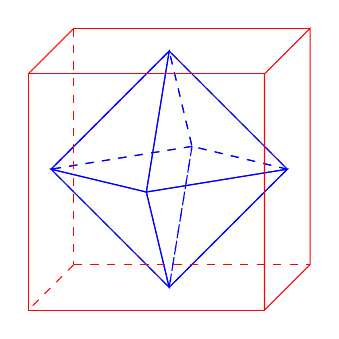
\begin{tikzpicture}[z = -5.5, scale = 1.5]
    \coordinate (O1) at (0, 0, -1);
    \coordinate (O2) at (-1, 0, 0);
    \coordinate (O3) at (0, 0, 1);
    \coordinate (O4) at (1, 0, 0);
    \coordinate (O5) at (0, 1, 0);
    \coordinate (O6) at (0, -1, 0);

    \draw [draw = blue, dashed] (O1) -- (O2) -- (O5) -- cycle;
    \draw [draw = blue, dashed] (O4) -- (O1) -- (O5) -- cycle;
    \draw [draw = blue, dashed] (O1) -- (O2) -- (O6) -- cycle;
    \draw [draw = blue, dashed] (O4) -- (O1) -- (O6) -- cycle;
    \draw [draw = blue] (O2) -- (O3) -- (O5) -- cycle;
    \draw [draw = blue] (O3) -- (O4) -- (O5) -- cycle;
    \draw [draw = blue] (O2) -- (O3) -- (O6) -- cycle;
    \draw [draw = blue] (O3) -- (O4) -- (O6) -- cycle;

    \coordinate (C1) at (-1, -1, -1);
    \coordinate (C2) at (-1, -1, 1);
    \coordinate (C3) at (-1, 1, 1);
    \coordinate (C4) at (-1, 1, -1);
    \coordinate (C5) at (1, -1, -1);
    \coordinate (C6) at (1, -1, 1);
    \coordinate (C7) at (1, 1, 1);
    \coordinate (C8) at (1, 1, -1);

    \draw [draw = red, dashed] (C1) -- (C2);
    \draw [draw = red] (C2) -- (C3);
    \draw [draw = red] (C3) -- (C4);
    \draw [draw = red, dashed] (C4) -- (C1);
    \draw [draw = red] (C5) -- (C6) -- (C7) -- (C8) -- cycle;
    \draw [draw = red, dashed] (C1) -- (C5);
    \draw [draw = red] (C2) -- (C6);
    \draw [draw = red] (C3) -- (C7);
    \draw [draw = red] (C4) -- (C8);
  \end{tikzpicture}
\end{center}

\subsection{Dodecahedron (dual to Icosahedron) - Non examinable}

Let $D$ be the dodecahedron.

\begin{itemize}
    \item 12 regular pentagonal faces
    \item 30 edges
    \item 20 vertices
\end{itemize} 

Let $G^+ =$ group of rotations of $D$. \\
Let $F$ be a face of $D$.
\begin{align*}
    | \operatorname{Orb}_{G^+}(F)| &= 12 \\
    | \operatorname{Stab}_{G^+}(F) | &= 5 \text{ just rotating about face} \\
    \implies |G^+| &= 5 \times 12 = 60 \text{ by \Cref{thm:orbit}.}
\end{align*} 

There are five cubes embedded in $D$.

\begin{figure}
    \centering
    \includegraphics[height=5cm]{figures/07-cube-dodecahedron}
\end{figure} 

15 pairs of edges, 3 pairs per cube $\implies$ 5 cubes.

$G^+$ acts faithfully on cubes, giving us an injective map $\Phi : G^+ \to S_5$.
And $|G^+| = 60 \implies G^+ \cong A_5$ ($A_5$ is the only subgroup of order 60 of $S_5$).
The smallest non-abelian simple group comes up as the rotational group of a dodecahedron.

We can find the elements of $A_5$
\begin{itemize}
    \item Rotations through opposite faces - 5 cycles (6 axes, 4 elements per axis giving 24 elements).
    \item Rotations through opposite vertices - 3 cycles.
    \item Rotations through opposite edges - double transpositions (15 such).
\end{itemize} 